\documentclass{article}
\usepackage{amsmath}
\usepackage{graphicx}
\usepackage[utf8]{inputenc}
\usepackage{parskip}

\setcounter{secnumdepth}{0}

\date{}
\author{Kaan Aksoy | Feb 15, 2020}

\begin{document}

\maketitle
\section{Principle of Inclusion and Exclusion}
\subsection{Overview}

The Principle of Inclusion and Exclusion (\textit{PIE}) is 
useful for counting the number of elements in the union 
of multiple sets. In particular, it is useful for the union 
of sets that are not mutually exclusive, where adding the 
number of elements in each set does not give the correct value.

For example, consider the sets $A = \{1,2,3\}$ and $B = \{3, 4, 5\}$. In this case, adding the number of elements in each set 
gives $6$, when in reality $\lvert A \cup B \rvert = 4$. 

Below, cases of \textit{PIE} for $2$, $3$, and $n$ sets will be described.

\subsection{\textit{PIE} for 2 sets}

For the case with $2$ sets, \textit{PIE} is often called the \textit{Addition Rule}, and can be stated as:

$$ |A \cup B| = |A| + |B| - |A \cap B|$$

The subtraction on the right side of the equation is necessary 
to prevent double-counting of $A \cap B$, which can be seen visually in the diagram below:

\begin{figure}[h]
\centering
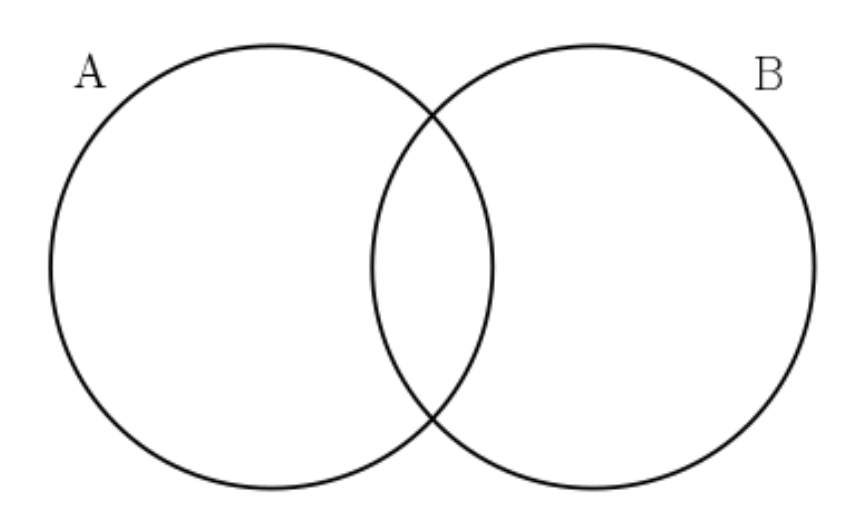
\includegraphics[width=5cm]{VennDiagram2}
\caption{Two sets that are not mutually exclusive}
\end{figure}

\subsection{\textit{PIE} for 3 Sets}

For $3$ sets, \textit{PIE} can be stated as:

$$ |P \cup M \cup F| = |P| + |M| + |F| - 
|P \cap M| - |P \cap F| - |M \cap F| 
+ |P \cap M \cap F| $$

In this equation, the first $3$ subtractions eliminate 
repeated countings of the intersection of every pair of sets. 
However, in the process, the intersection of 
all $3$ sets is wrongly ignored, which 
is why $|P \cap M \cap F|$ must be added.

\begin{figure}[h]
\centering
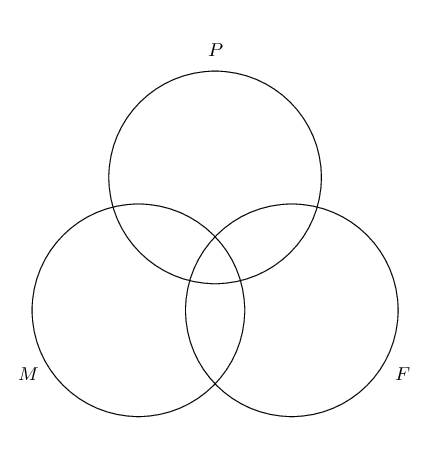
\includegraphics[width=5cm]{VennDiagram3}
\caption{Three sets that are not mutually exclusive}
\end{figure}

\subsection{\textit{PIE} for \textit{n} Sets}

Generalizing from \textit{PIE} for $2$ and $3$ sets, \textit{PIE} for $n$ sets can be written as:

$$
\left\lvert \bigcup_{i=1}^{n} A_{n} \right\rvert ={} 
\sum_{i=1}^{n} \lvert A_{i} \rvert
\, - \sum_{1 \leq i \leq j \leq n} \lvert A_{i} \cap A_{j} \rvert 
\, + \sum_{1 \leq i \leq j \leq k \leq n} \lvert A_{i} \cap A_{j} \cap A_{k} \rvert 
\, - \ldots
\, + (-1)^{n-1} \lvert A_{1} \cap A_{2} \cap \ldots \cap A_{n} \rvert
$$

\subsection{Example Problem 1}
How many permutations of $26$ letters (a-z) do not contain any 
of: fish, rat, bird?

Let $F$, $R$, and $B$ be sets of permutations that contain 
fish, rat, and bird, respectively. We begin by computing the 
cardinality of these sets, as well as their intersections:

\begin{equation*}
\begin{split}
|F| &= (26 - 4 + 1)! = 23! \\
|R| &= (26 - 3 + 1)! = 24! \\
|B| &= (26 - 4 + 1)! = 23! \\
|F \cap R| &= (26 - 4 - 3 + 1 + 1) = 21! \\
|F \cap B| &= 0 \\
|R \cap B| &= 0 \\
|F \cap R \cap B| &= 0 \\
\end{split}
\end{equation*}

The last $3$ cardinalities are $0$ because the words contain 
the same letters and cannot appear in the same permutation. 
Then, we apply \textit{PIE} to calculate the number 
of permutations containing fish, rat, or bird:

\begin{equation*}
\begin{split}
|F \cup R \cup B| &= |F| + |R| + |B| - 
|F \cap R| - |F \cap B| - |R \cap B| 
+ |F \cap R \cap B| \\
&= 23! + 24! + 23! - 21!
\end{split}
\end{equation*}

Finally, we subtract this value from the total number 
of permutations, giving $ 26! - \left[ (2)23! + 24! - 21! \right] $ as the final answer.

\subsection{Example Problem 2}

How many ways can you seat n couples at a very 
long dinner table with seats 1..2n such that no 
couple sits next to each other.

\end{document}